\CHAPTER{Introduction}
\label{chapter1}

\section{Gravitational Waves}

Almost all of humanity's knowledge of the universe is derived from
observations of electromagnetic waves.  The effort to detect
gravitational waves seeks to expand this knowledge by observing an
entirely different field, and to further verify the correctness of the
theory of general relativity.

Any theory of gravity that avoids instantaneous action at a distance
must feature some kind of gravitational waves.  Even Newtonian gravity
can be modified to account for propagation delays from massive bodies
that are the sources of attraction\cite{Schutz1984Gravitational}.
Gravity as we know it, however, is described by the general theory of
relativity.  In general relativity, spacetime is treated as a
four-dimensional manifold with some intrinsic curvature.  This
curvature is generated by the presence of mass and energy.  In the
absense of forces, particles follow geodesic trajectories on this
manifold.  Thus, in the quintessential words of John Wheeler(?),
``Space tells matter how to move, matter tells space how to curve.''

This relationship between matter and curvature is made formal through
the Einstein field equation, which equates (up to units) the Einstein
tensor ($\mathsf{G}$), encoding curvature, with the
Stress-Energy tensor ($\mathsf{T}$), encoding the matter and energy
contents:
\begin{equation}
\mathsf{G} = \frac {8\pi G}{c^4} \mathsf{T}
\end{equation}
where $G$ is (Newton's) universal gravitational constant and $c$ is
the speed of light.

To perform calculations, we typically need to work in some coordinate
basis.  Thus one will work with $G_{\mu\nu}$, where $\mu$ and $\nu \in
{0,1,2,3}$ are coordinate indices.  In this notation, the Einstein
tensor is given by $G_{\mu\nu} = R_{\mu\nu} - \frac{1}{2} R
g_{\mu\nu}$, where $R_{\mu\nu}$ is the Ricci curvature tensor, $R$ is
the Ricci scalar, and $g_{\mu\nu}$ is the spacetime metric.  The
metric plays a central role here, as it both encodes the curvature and
implicitly defines the coordinate system.

\begin{figure}
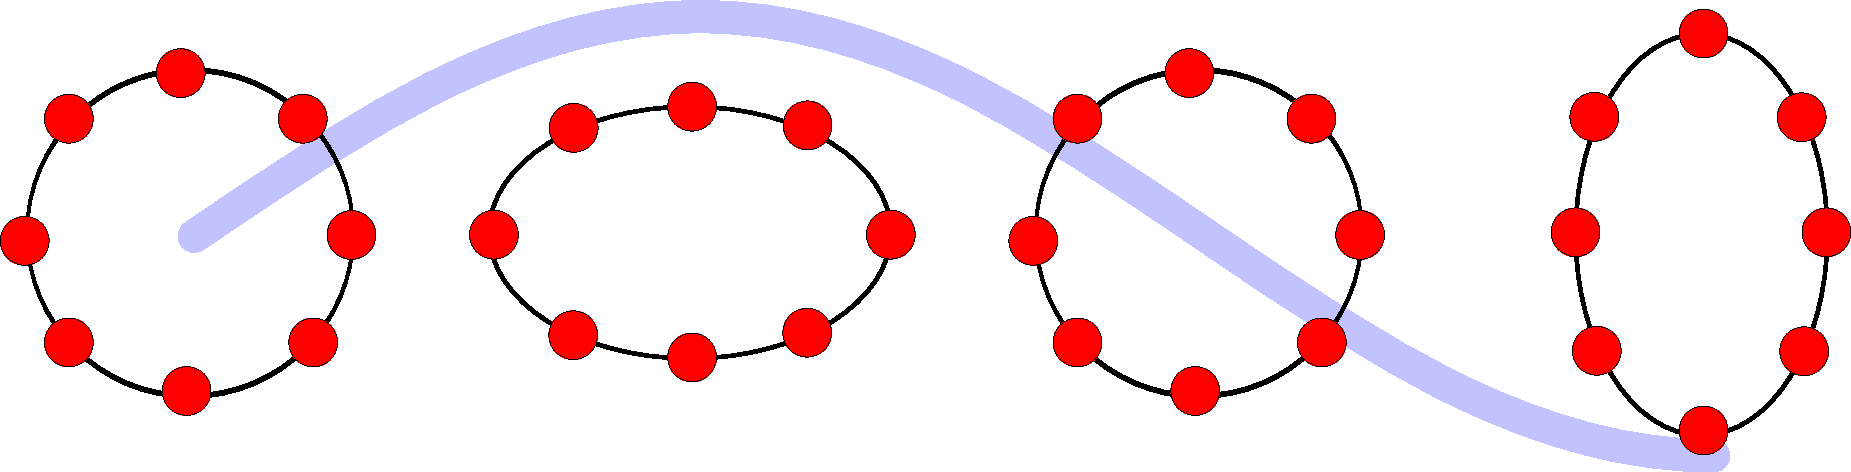
\includegraphics[width=\columnwidth]{chapter1/figures/gwave.pdf}
\caption[Effect of a gravitational wave on a ring of test
  particles]{\label{fig:gwave-effect}Effect of a gravitational wave
  (traveling into or out of the page) on a ring of non-interacting
  inertial test particles.}
\end{figure}

To reveal the mechanism of gravitational waves, we are interested in
vacuum ($\mathsf{T}=0$) solutions of the Einstein field equations in
the weak-field limit.  In the weak-field limit, we can write the
metric $g_{\mu\nu}$ as the sum of the flat-space Minkowski metric
$\eta_{\mu\nu}$ and a small perturbation $h_{\mu\nu}$:
$$g_{\mu\nu} = \eta_{\mu\nu} + h_{\mu\nu}$$ This is the regime of
linearized gravity.  Calculating out the Einstein field equation
keeping only terms of first-order in $h$ and choosing the
transverse-traceless gauge, one finds (see Sean Carroll's lucid
exposition in \cite{Carroll1997Lecture} for the details) a wave
equation for $h$:
$$\left(\nabla^2 - \frac{1}{c^2}\frac{\partial^2}{\partial t^2}\right)h_{\mu\nu} = 0$$
where $h_{\mu\nu}$ has, for a wave propagating along the $z$ axis, the form:
$$ [\mathsf{h}] = \left(
\begin{array}{cccc}
0 & 0 &  0 & 0 \\
0 & a &  b & 0 \\
0 & b & -a & 0 \\ 
0 & 0 &  0 & 0 
\end{array}
 \right)$$
Here we see several of the essential points of gravitational waves:
\begin{itemize}
\item There are two independent components (polarizations)
\item They travel at the speed of light 
\item They are manifest as a transverse tidal force on inertial objects
\end{itemize}

The amplitude of gravitational waves is quantified as the effective
strain exerted on inertial test-masses.

\section{The Hulse-Taylor Pulsar}

Gravitational waves have not yet been directly detected, but very
strong indirect evidence exists.  Perhaps the strongest evidence is
the Hulse-Taylor
pulsar~\cite{Hulse1975Discovery,Weisberg2005Relativistic}--a
remarkable discovery of a binary star system in which one of the
constituents is pulsar PSR B1913+16. The binary system is expected to
radiate energy away into gravitational waves, causing its orbit to
decay.  The pulsar reveals the orbital parameters of the binary
system, in particular its orbital period. Measurement of the orbital
period through pulsar tracking over 30 years shows that the orbit is
decaying exactly as predicted by general relativity.

Another binary system containing pulsars was discovered in 2004.  In
this system \emph{both} objects are
pulsars. \cite{Lyne2004DoublePulsar,Kramer2006Tests}

\section{Sources of Gravitational Waves}
Any system of mass accelerating in the quadrupolar or higher moments
will radiate energy into gravitational waves.  The effect is so weak,
however, that only some of the universe's more cataclysmic events have
a chance of producing waves observable on earth.

Anticipated sources of gravitational waves can be conveniently
categorized as \emph{continuous} or \emph{transient}, and as
\emph{modeled} or \emph{unmodeled}.  There is some overlap in this
division.  Sources are paired with associated search efforts.

\begin{itemize}

\item \textbf{compact binary coalescence} --- Pairs of compact objects
  (black holes or neutron stars) in binary orbits are expected to lose
  energy through gravitational waves, causing the orbit to decay until
  the objects finally begin to interact and merge into a single
  object.  This inspiral process will generate a characteristic chirp
  signal, followed by the complex merger process and then ringdown.

\item \textbf{continuous wave} --- Rapidly spinning objects will
  generate essentially monochromatic signals, which are in turn
  doppler-shifted by the relative motion of the Earth and the source.
  This is sometimes called the pulsar search, since the primary source
  in this category is expected to be rapidly spinning neutron stars
  (such as pulsars).  The search, in turn, is divided into searches
  for known pulsars and unknown pulsars.  Pulsars which are known
  electromagnetically can be targetted directly, whereas unknown
  pulsars require a brute-force search of the parameter space.

  Currently this is attacked in part through the distributed computing
  project Einstein@Home.  One nicety of the pulsar search is that the
  process works equally well for analyzing radio telescope data--this
  has been done, resulting in the discovery of several previously
  unknown radio pulsars\cite{Knispel2010Pulsar}.  It is an open
  problem to find a more efficient search algorithm.

\item \textbf{bursts} --- Transient cataclysmic events such as
  supernovae will generate bursts of gravitational waves whose
  waveforms is not known in advance.  

\item \textbf{stochastic background} --- In the same manner as the
  cosmic microwave background radiation, a cosmological background of
  gravitational waves is expected to exist.  This is perhaps the most
  exotic anticipated source of gravitational waves, since its
  detection will inform us of the state of the universe at an age far
  earlier than has yet been probed.  Sadly, the cosmological
  background is almost certainly too weak to detect in the forseeable
  future.

  The cacophony of unresolved astrophysical sources will also combine
  to produce a gravitational wave stochastic background.   

  The stochastic background search is fully coherent.  In its simplest
  form, the search simply computes the correlation between pairs of
  gravitational wave detectors.  This can be done in either an all-sky
  search or in a sky-position-dependent search.  Typically, some
  power-law gravitational wave spectrum is assumed.

\end{itemize}

Improvements in search sensitivity can be achieved by incorporating
knowledge of the expected signal waveform or spectrum; integrating
over a long period of time (for continuous sources); and by looking
for coincidence or coherence between multiple detectors.

The global network of gravitational wave detectors is operated as a
sensor array, an interferometer composed of many interferometers.

\section{Detectors}
Gravitational waves couple to both light and matter.

\begin{figure}
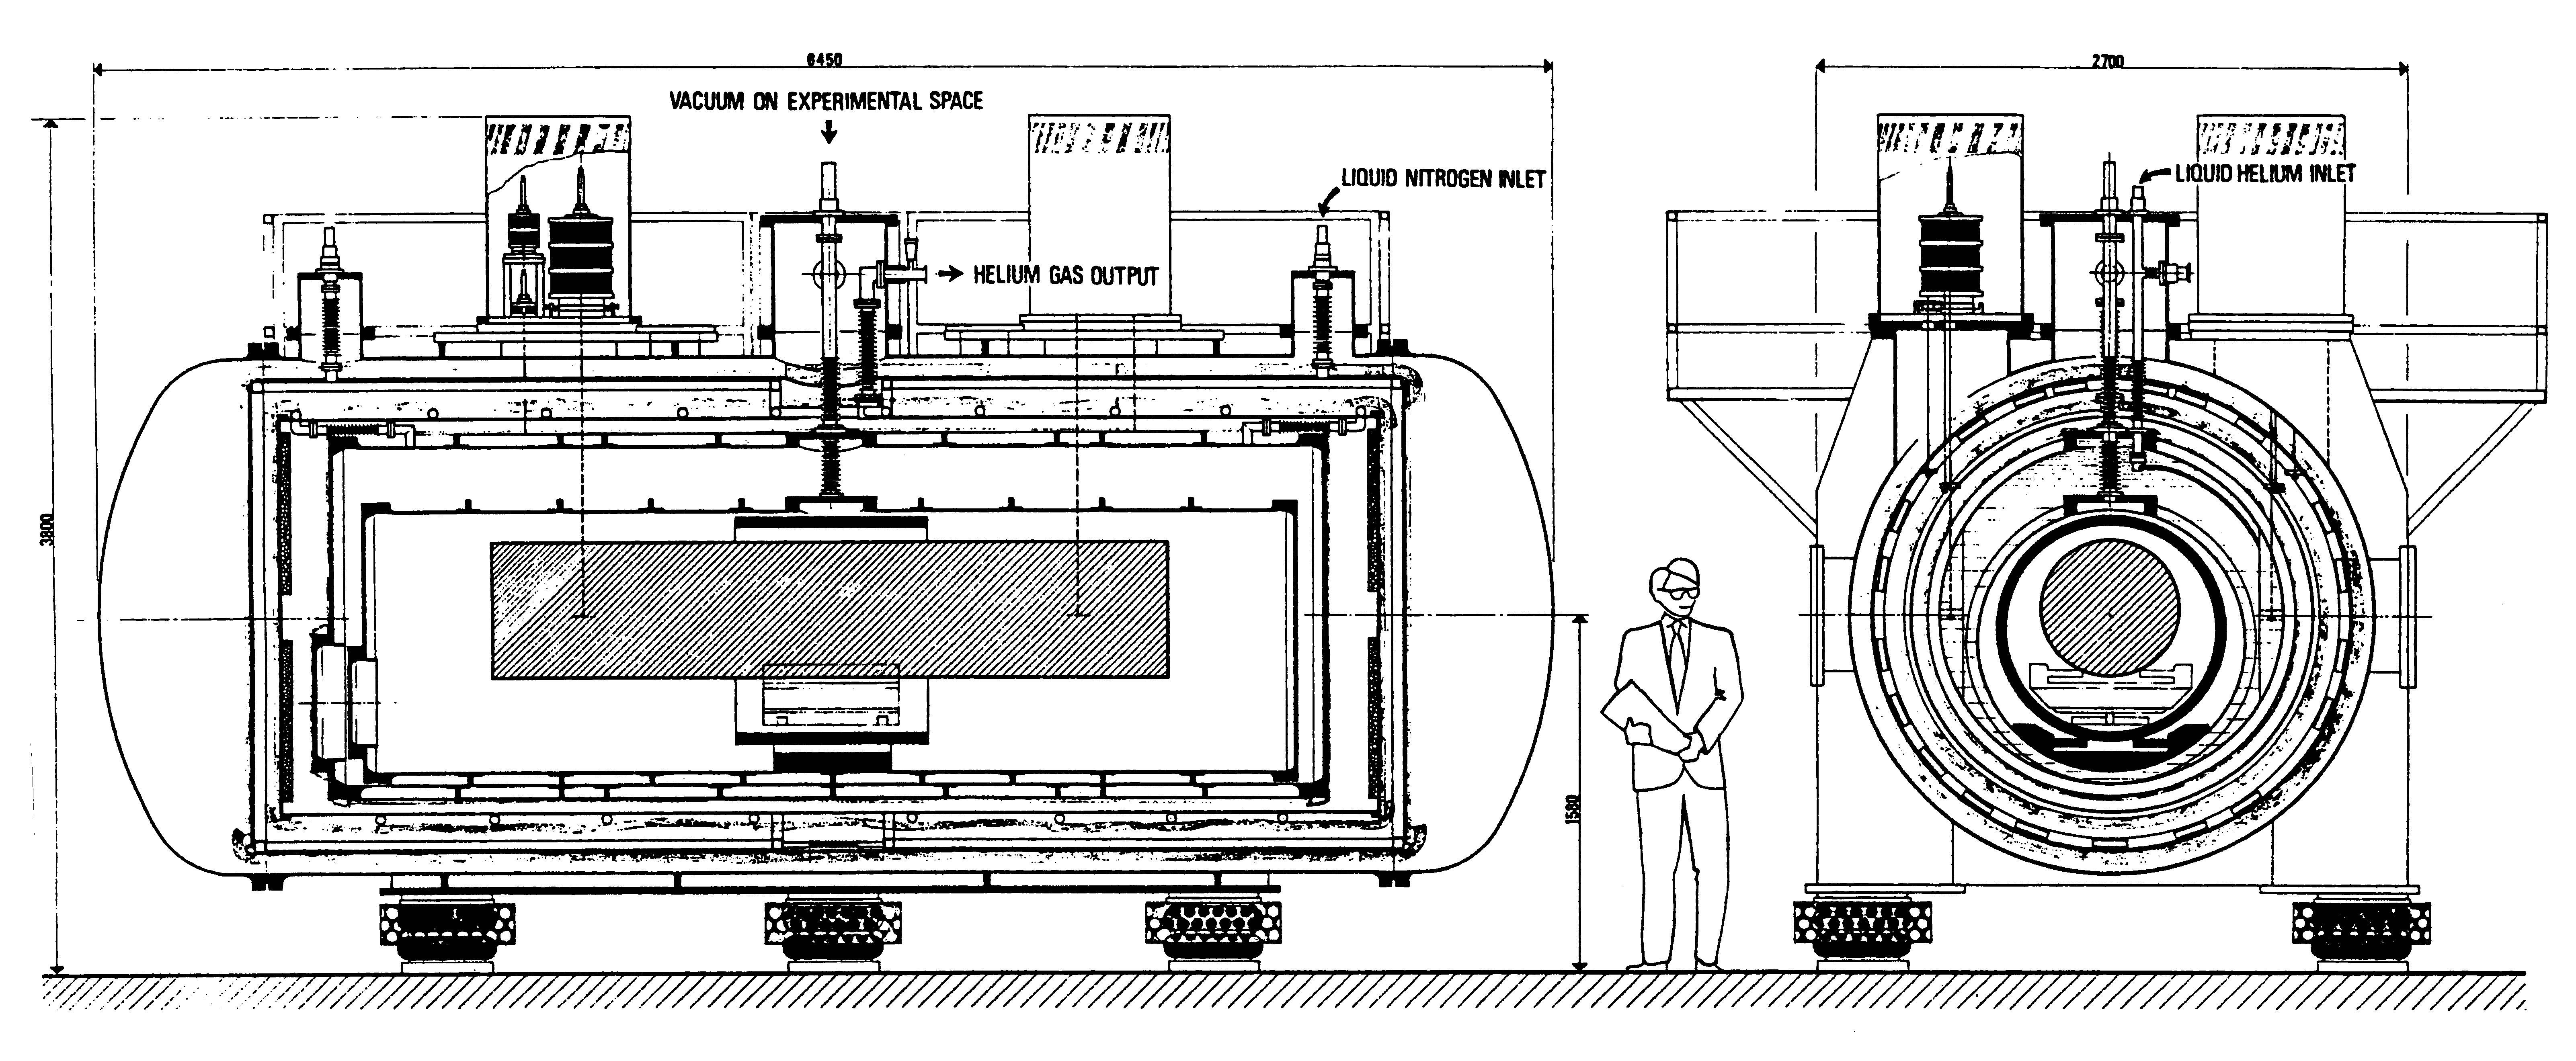
\includegraphics[width=\columnwidth]{chapter1/figures/explorer.png}
\caption[EXPLORER bar detector]{\label{fig:explorer-bar}Depiction of the cryostat of the
  EXPLORER bar detector, which operated \checkme{somewhere} for
  \checkme{some time}.  Illustration adapted from \checkme{a
    reference}.}
\end{figure}

The first attempts to detect gravitational waves used resonant bar
detectors.  In such a detector, a large cylinder of a metal alloy with
a very high mechanical Q-factor is suspended in a vacuum chamber and
cooled to cryogenic temperatures.  A passing gravitational wave
couples mechanical energy into the bar, ringing up the fundamental
mechanical mode of the bar.  Sensitive detectors (latter bars used
SQUIDs) read out this mechanical displacement.  Resonant bars are
inherently narrow-band devices, sensitive to gravitational waves
within a narrow linewidth about their fundamental resonance.

Bar detectors do have the advantage that they are small enough that
they can be moved or re-oriented.  The ALLEGRO bar detector at LSU~\cite{Mauceli1996Allegro} was
rotated to modulate its overlap function with the nearby LIGO
Livingston observatory.%\cite{Abbott2007First}

\subsection{Laser interferometers}

Laser interferometers are now the instrument of choice in the search
for gravitational waves.  A gravitational wave will modulate the
optical path length of light traveling transversely through it between
inertial test masses.  This path length modulation can be detected by
a laser interferometer.  The operation of laser interferometer
gravitational wave detectors is the focus of this work and is detailed
in the following chapters.

In terrestrial interferometers, large\footnote{10 kg in Initial LIGO,
  40 kg in Advanced LIGO} glass cylinders serve as both super-polished
mirrors and inertial test masses.  These optics are hung as pendula to
allow inertial freedom of the pendular resonance frequency.

References to cite in this section: \cite{Weiss1972Electromagnetically,Forward1978Wideband}

\subsection{Other detectors}

There are a few other mechanisms by which gravitational waves may be
detected.

Pulsars serve as extremely reliable clocks, beaming a sequence of
pulses towards earth whose arrival times can typically be predicted to
better than a microsecond.  The path of the electromagnetic waves
traveling from the pulsar to earth acts in some ways like an arm of a
laser interferometer: gravitational waves passing transversely to the
Earth-Pulsar baseline will modulate the optical path length, producing
perturbations in the arrival time of the pulsar pulses--perturbations
which are correlated between observations of distinct pulsars. Pulsar
timing arrays seek to analyze these correlated residuals to find
evidence of gravitational waves;
Hobbs~\cite{Hobbs2009International} anticipates that pulsar timing
analysis will yield detections of gravitational waves in the nanohertz
regime (period 3-30 years) in the next 5-10 years.

Primordial gravitational waves will also leave their imprint on the
polarization of the cosmic microwave background radiation.  Many CMB
polarization experiments are currently underway, searching for the
faint ``B-modes'' in the microwave polarization.

\section{LIGO}

Ground was broken on the first of the two LIGO observatories in 1994.
After years of construction and then detector commissioning, the three
detectors at the two observatories reached their design sensitivity in
2004.  Having reached this milestone, the attention turned to
collecting data for astrophysical observation rather than instrument
development.  By October 2007, the LIGO project accomplished the goals
of what is now known as ``initial LIGO,'' having collected 1 year of
observational data with all three detectors online simultaneously.

It had always been intended that this initial generation of LIGO would
be followed by a programme of improvements.  The next generation of
LIGO detectors is ``Advanced LIGO,'' which will feature significantly
more effective (and more complex) seismic isolation, an increase of
$20\times$ in laser power, in addition to other improvements.

Rather than spend the entire time before the onset of Advanced LIGO
taking observational data in the Initial LIGO configuration, it was
decided to implement an intermediate series of upgrades in a project
that came to be called ``Enhanced
LIGO''\cite{Adhikari2006Enhanced,T050252,JoshSmithEnhancedAdvanced}.
The goals of enhanced LIGO were to both increase the changes of an
early discovery (by increasing the detector sensitivity), and to gain
early experience with Advanced LIGO technologies.

\subsection{Summary of changes made for Enhanced LIGO}

Detector upgrades during Enhanced LIGO included:
\begin{itemize}
\item An increase in laser power.  The initial LIGO laser, an Nd:YAG
  NPRO capable of producing $< 10$ Watts of laser power at a
  wavelength of 1064 nm, was replaced with the Advanced LIGO laser
  front-end, built by Laser-Zentrum Hannover, with an output power of 35 W.
\item The input optics were redesigned to handle the higher input
  power~\cite{Dooley2011Characterization,Quetschke2008ElectroOptic}.  
\item A new thermal compensation system was implemented to compensate
  for the greater amount of thermal lensing that would be induced by
  the higher operating power.
\item An output mode cleaner was installed, supported by a prototype
  of the advanced LIGO in-vacuum seismic isolation system
\item The Angular Sensing and Control system was redesigned to cope
  with angular instabilities introduced at high
  power~\cite{Sidles2006Optical,DooleyAngular}
\item Readout of the gravitational wave channel was changed from RF
  readout to DC readout.
\end{itemize}

\section{The Future}

It is hoped that Advanced LIGO, currently under construction, will
bring the first direct detection of gravitational waves and begin the
era of regular detection.

Several next-generation interferometers are in the works. 

The Einstein telescope~\cite{EinsteinTelescopeDesignStudy2011} is a
planned system of three interferometers with arms forming an
equilateral triangle, to be installed in tunnels deep under Europe.

In the meantime, technological development of terrestrial laser
interferometers is a vibrant field.  The Advanced detectors are
anticipated to be limited almost everywhere by quantum mechanical
noises, making gravitational wave detectors a verdant field for work
in quantum optics.  The next generation of terrestrial gravitational
wave detectors will be limited by near-field gravity--``Newtonian
noise'' from density waves in the surrounding environment.  The ways
forward will be to move underground (where this effect is smaller);
measure, predict, and subtract the Newtonian noise contribution using
a seismic sensor array; or to move into space.

Going into space makes feasible the use of extraordinarily long arms
and yields complete freedom from terrestrial noise, allowing access to
very low frequency gravitational waves.  The Laser Interferometer
Space Antenna (LISA) design is composed of three spacecraft forming an
equilateral triangle, the whole constellation in solar orbit.  These
spacecraft will house truly inertial test-masses, floating within an
internal vacuum enclosure while external microthrusters keep the
spacecraft centered around the test mass.  The gravitational wave
channel is derived using time-delay interferometery.  The proposed
LISA design is sensitive to gravitational waves in the range $10^{-4}$
to $10^{-1}$ Hz (period of 3 hours down to 10 seconds).

\section{This Dissertation}

This dissertation describes the implementation of DC readout and an
output mode cleaner during Enhanced LIGO.

The state of the LIGO detectors before these modifications is
described in \cite{S5InstrumentPaper} as well as numerous PhD
dissertations, notably Rana Adhikari's \cite{RanaThesis} and and
Stefan Ballmer's \cite{Ballmer2006LIGO}.  Robert Ward's dissertation
details the implementation and evaluation of DC readout at the LIGO 40
meter prototype interferometer in Pasadena \cite{RobWardThesis}.

In Chapter 2, I explain the principles and practice behind the
sensitivity of the LIGO detectors.  I show how the machine converts
gravitational wave-induced phase modulation into a modulated optical
field while offering a large amount of immunity to other effects.

In Chapter 3, I describe DC readout.

Chapter 4 introduces the Output Mode Cleaner, its design and control,
and the general idea of mode cleaners.

Finally, in Chapter 5, I present results demonstrating the performance
of this system.

Additional derivations and background are given in the appendicies.
